\documentclass[uplatex,dvipdfmx]{jsarticle}
\usepackage{amssymb}
\usepackage{amsmath}
\usepackage{amsthm}
\usepackage{framed}
\usepackage{braket}
\usepackage{bm}
\usepackage{mathrsfs}
\usepackage{mathabx}
\usepackage{tocloft}
\usepackage[dvipdfmx]{graphicx}
\usepackage{tikz}
\usepackage{url}
\usepackage{color}
\usepackage{xifthen}
\usepackage{xcolor}
\usepackage{framed}
\usepackage{mathtools}
\usepackage[explicit]{titlesec}
\usepackage{stmaryrd}
\usepackage[all]{xy}
\usepackage{geometry}
\geometry{left=35mm,right=35mm,top=35mm,bottom=35mm}

\usetikzlibrary{positioning}
\usetikzlibrary{calc}
\usetikzlibrary{decorations.pathreplacing}
\usetikzlibrary{cd}

\newcommand{\scrN}{\mathcal{N}}
\newcommand{\scrC}{\mathcal{C}}
\newcommand{\scrI}{\mathcal{I}}
\newcommand{\scrJ}{\mathcal{J}}
\newcommand{\N}{\mathbb{N}}
\newcommand{\Z}{\mathbb{Z}}
\renewcommand{\P}{\mathbb{P}}
\newcommand{\B}{\mathbb{B}}
\newcommand{\Q}{\mathbb{Q}}
\newcommand{\R}{\mathbb{R}}
\newcommand{\C}{\mathbb{C}}
\newcommand{\range}{\operatorname{ran}}
\newcommand{\dom}{\operatorname{dom}}
\newcommand{\append}{{}^\frown}
\newcommand{\boldsig}{\boldsymbol{\Sigma}}
\newcommand{\boldpi}{\boldsymbol{\Pi}}
\newcommand{\bolddelta}{\boldsymbol{\Delta}}
\newcommand{\Ordinals}{\mathrm{On}}
\newcommand\forces{\Vdash}
\newcommand\notforces{\nVdash}
\newcommand{\cl}{\operatorname{cl}}
\newcommand{\intr}{\operatorname{int}}
\newcommand{\rank}{\operatorname{rank}}
\newcommand{\Pow}{\mathcal{P}}
\newcommand{\OR}{\mathbin{\text{または}}}
\newcommand{\AND}{\mathbin{\text{かつ}}}
\newcommand{\GP}{\operatorname{GP}}
\newcommand{\non}{\operatorname{non}}
\newcommand{\cov}{\operatorname{cov}}
\newcommand{\add}{\operatorname{add}}
\newcommand{\cof}{\operatorname{cof}}
\newcommand{\nul}{\mathcal{N}}
\newcommand{\meager}{\mathcal{M}}
\newcommand{\frakt}{\mathfrak{t}}
\newcommand{\frakc}{\mathfrak{c}}
\newcommand{\frakb}{\mathfrak{b}}
\newcommand{\frakd}{\mathfrak{d}}
\newcommand{\all}{\mathrm{all}}
\newcommand{\ZFC}{\mathrm{ZFC}}
\newcommand{\ZF}{\mathrm{ZF}}
\newcommand{\AD}{\mathrm{AD}}
\newcommand{\DC}{\mathrm{DC}}
\newcommand{\GCH}{\mathrm{GCH}}
\newcommand{\proj}{\operatorname{proj}}
\newcommand{\cf}{\operatorname{cf}}
\newcommand{\EUB}{\mathsf{EUB}}
\newcommand{\COB}{\mathsf{COB}}
\newcommand{\relR}{\mathbf{R}}
%\newcommand{\Pa}{\mathbb{P}^\mathrm{pre}}
\newcommand{\crit}{\operatorname{crit}}
\newcommand{\supp}{\operatorname{supp}}
\newcommand{\Eor}{\mathbb{E}}
\newcommand{\ve}{\varepsilon}
\newcommand{\on}{\mathord\upharpoonright}


\newcommand{\Pa}{\mathbb{P}^5}
\newcommand{\PaB}{\mathbb{P}^{*,5}}
\newcommand{\Pai}{\mathbb{P}^i}
\newcommand{\Paj}{\mathbb{P}^j}
\newcommand{\Paell}{\mathbb{P}^\ell}
\newcommand{\Paip}{\mathbb{P}^{i+1}}
\newcommand{\PaVI}{\mathbb{P}^6}
\newcommand{\PaVII}{\mathbb{P}^7}
\newcommand{\PaVIII}{\mathbb{P}^8}
\newcommand{\PaIX}{\mathbb{P}^9}


\newcommand{\mye}{*+[F.]{\phantom{\lambda}}}
\newcommand{\myb}{*{\phantom{\lambda}}}

\newcommand{\covnull}{\cov(\mathcal N)}
\newcommand{\cofnull}{\cof(\mathcal N)}
\newcommand{\addnull}{\add(\mathcal N)}
\newcommand{\nonnull}{\non(\mathcal N)}
\newcommand{\covmeager}{\cov(\mathcal M)}
\newcommand{\cofmeager}{\cof(\mathcal M)}
\newcommand{\addmeager}{\add(\mathcal M)}
\newcommand{\nonmeager}{\non(\mathcal M)}

\DeclarePairedDelimiter\abs{\lvert}{\rvert}
\newcommand{\seq}[1]{{\langle#1\rangle}}
\DeclarePairedDelimiterX{\norm}[1]{\lVert}{\rVert}{#1}
\newcommand{\truth}[1]{\llbracket #1 \rrbracket}

\renewcommand\emptyset{\varnothing}
\renewcommand\subset{\subseteq}
\renewcommand{\setminus}{\smallsetminus}


\theoremstyle{definition}
\newtheorem{thm}{定理}
\newtheorem*{thm*}{定理}
\newtheorem{defi}[thm]{定義}
\newtheorem*{defi*}{定義}
\newtheorem{lem}[thm]{補題}
\newtheorem*{lem*}{補題}
\newtheorem{fact}[thm]{事実}
\newtheorem*{fact*}{事実}
\newtheorem{prop}[thm]{命題}
\newtheorem*{prop*}{命題}
\newtheorem{exm}[thm]{例}
\newtheorem*{exm*}{例}
\newtheorem{rmk}[thm]{注意}
\newtheorem*{rmk*}{注意}
\newtheorem{cor}[thm]{系}
\newtheorem*{cor*}{系}
\newtheorem*{notation*}{記法}
\newtheorem{prob}[thm]{問題}
\newtheorem{conj}[thm]{予想}
\newtheorem{property}[thm]{性質}
\newtheorem{assumption}[thm]{仮定}
\newtheorem{observation}[thm]{観察}
\renewcommand{\proofname}{証明}


\newcommand{\todo}[1][]{%
	\ifthenelse{\equal{#1}{}}{%
		\textcolor{red}{[TODO]}%
	}{%
		\textcolor{red}{[TODO: #1]}%
	}%
}


\usepackage[backend=biber,style=alphabetic,sorting=nty,doi=false,isbn=false,url=false,eprint=true]{biblatex}
\addbibresource{cichonsmaximum.bib}
\renewbibmacro{in:}{}

\title{Cichoń's maximumの証明}
\author{後藤 達哉}

\begin{document}
	\maketitle
	
	
	\tableofcontents
	
	\section{イントロダクション}
	
	実数全体の集合$\R$をLebesgue測度0集合たちで覆うには,それらが最低何個必要かという問いを考える.Lebesgue測度0集合の可算和はLebesgue測度0だから可算個では足りない.一方,$\bigcup_{r \in \R} \{r\} = \R$だから連続体濃度個あれば十分である.
	これで非可算かつ連続体濃度以下とわかるわけだが,ここで問いを終えてしまうのはもったいない.連続体濃度の下に非可算基数が存在することもありえると分かっているからだ.
	そこで問の答えを
	\[
	\cov(\nul) = \min \{ \abs{\mathcal{A}}  : \mathcal{A}\text{はルベーグ測度}0\text{集合の族で}\bigcup \mathcal{A} = \R \}
	\]
	とおいて,これがいろんな集合論のモデルでどうなっているのか調べよう.
	また,他の似たような問いの答えを文字でおいてそれらの間の関係を調べよう:ZFCの範囲内で大小関係がつくのか,等しいのか,ZFCで等しいことを証明できないなら実際にどんなモデルで破れているのか.これが\textbf{基数不変量}の研究である.
	
	基数不変量という言葉に厳密な定義はないが,「実数の構造によって定義される基数」のことであり,その多くは$\aleph_1$以上$2^{\aleph_0}$以下であることが証明される.
	
	いくつかの基数不変量を定義しよう.
	
	$2^\omega$上のイデアル$\mathcal{I}$に対して
	\begin{itemize}
		\item $\add(\mathcal{I}) = \min \{ \abs{\mathcal{J}} : \mathcal{J} \subset \mathcal{I}, \bigcup \mathcal{J} \not \in \mathcal{I}  \}$
		\item $\cov(\mathcal{I}) = \min \{ \abs{\mathcal{J}} : \mathcal{J} \subset \mathcal{I}, \bigcup \mathcal{J} = 2^\omega  \}$
		\item $\non(\mathcal{I}) = \min \{ \abs{A} :  A\subset 2^\omega, A \not \in \mathcal{I} \}$
		\item $\cof(\mathcal{I}) = \min \{ \abs{\mathcal{J}} :  \mathcal{J} \subset \mathcal{I}, (\forall A \in \mathcal{I})(\exists B \in \mathcal{J})(A \subset B) \}$
	\end{itemize}
	とおく.
	これらにルベーグ測度$0$集合のイデアル$\nul$,痩せ集合のイデアル$\meager$を代入したものが考察の対象である.
	
	また,
	\begin{itemize}
		\item $\frakd = \min \{\abs{F} : F \subset \omega^\omega, (\forall f \in \omega^\omega)(\exists g \in F) (f \le^* g) \}$.
		\item $\frakb = \min \{\abs{F} : F \subset \omega^\omega, \neg (\exists f \in \omega^\omega)(\forall g \in F) (g \le^* f) \}$.
	\end{itemize}
	という基数不変量も考えられる.$\frakd$はdominating number,$\frakb$はbounding numberと呼ばれる.
	
	以上の10個の基数不変量のZFCで示せる大小関係については以下の図式が知られていて,Cichońの図式と呼ばれる.
	
	\[
	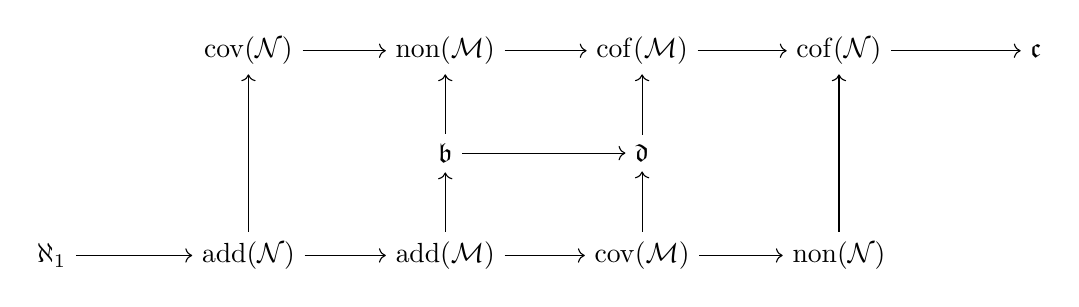
\begin{tikzpicture}
		\newcommand{\w}{2.5}
		\newcommand{\h}{1.3}
		
		\node (aleph1) at (-\w, 0) {$\aleph_1$};
		
		\node (addN) at (0, 0) {$\add(\nul)$};
		\node (covN) at (0, \h*2) {$\cov(\nul)$};
		
		\node (addM) at (\w, 0) {$\add(\meager)$};
		\node (b) at (\w, \h) {$\mathfrak{b}$};
		\node (nonM) at (\w, \h*2) {$\non(\meager)$};
		
		\node (covM) at (\w*2, 0) {$\cov(\meager)$};
		\node (d) at (\w*2, \h) {$\mathfrak{d}$};
		\node (cofM) at (\w*2, \h*2) {$\cof(\meager)$};
		
		\node (nonN) at (\w*3, 0) {$\non(\nul)$};
		\node (cofN) at (\w*3, \h*2) {$\cof(\nul)$};
		
		\node (c) at (\w*4, \h*2) {$\frakc$};
		
		\draw[->] (aleph1) to (addN);
		\draw[->] (addN) to (covN);
		\draw[->] (addN) to (addM);
		\draw[->] (covN) to (nonM);	
		\draw[->] (addM) to (b);
		\draw[->] (b) to (nonM);
		\draw[->] (addM) to (covM);
		\draw[->] (nonM) to (cofM);
		\draw[->] (covM) to (d);
		\draw[->] (d) to (cofM);
		\draw[->] (b) to (d);
		\draw[->] (covM) to (nonN);
		\draw[->] (cofM) to (cofN);
		\draw[->] (nonN) to (cofN);
		\draw[->] (cofN) to (c);
	\end{tikzpicture}
	\]
	ここで矢印$A \to B$は$A \le B$をZFCで証明できることを意味する.
	また$\add(\meager) = \min \{ \cov(\meager), \frakb \}$かつ$\cof(\meager) = \max \{ \non(\meager), \frakd \}$がZFCで証明できる.
	
	Cichońの図式に表示されている基数不変量以外にもBlassの図式と呼ばれる図式の基数不変量:$\mathfrak{m}, \mathfrak{p}, \mathfrak{h}, \mathfrak{g}, \mathfrak{s}, \mathfrak{e}, \mathfrak{r}, \mathfrak{a}, \mathfrak{u}, \mathfrak{i}$などもある.しかし,本稿ではこれらには焦点を当てない.
	
	\begin{table}[p]\label{table:history}
		\caption{Cichońの図式の歴史}
			\begin{tabular}{@{} l|l|p{8cm}}
			年     & 人物                                & 出来事                                                                                                                                                       \\ \hline
			1875年 & du Bois-Reymond & $\aleph_0 < \frakb$の証明 \\ \hline
			1891年 & Cantor & $\aleph_0 < \frakc$の証明 \\ \hline
			1938年 & Rothberger                        & $\cov(\meager) \le \non(\nul)$と$\cov(\nul)\le\non(\meager)$の証明                                                                                            \\ \hline
			1963年 & Cohen                             & 連続体仮説の独立性                                                                                                                                                 \\ \hline
			1970年 & Martin--Solovay                   & Martinの公理およびその帰結の$\add(\nul)=\frakc>\aleph_1$の証明                                                                                                           \\ \hline
			1977年 & Truss                             & $\min\{\cov(\meager), \frakb\} \le \add(\meager)$の証明                                                                                                       \\ \hline
			1981年 & Miller                            & $\add(\meager) \le \min\{\cov(\meager), \frakb\}$の証明およびこの時点で知られていたモデルでのCichonの図式の中の基数不変量の値の決定,Kunen-Millerの表 (5x5マス) \\ \hline
			1984年 & Miller                            & $\add(\nul) \le \frakb$の証明; Kunen-Millerの表 (6x6マス)                                                                                                        \\ \hline
			1984年 & Bartoszyński                      & $\add(\nul) \le \add(\meager)$の証明                                                                                                                         \\ \hline
			1984年 & Fremlin                      & $\cof(\meager) = \max\{\non(\meager), \frakd\}$の証明; Cichoń's diagram登場                                                                                                                     \\ \hline
			1985年 & Raisonnier--Stern                 & $\cof(\meager) \le \cof(\nul)$の証明                                                                                                                         \\ \hline
			1989年 & Bartoszyński--Judah--Shelah       & $\mathrm{PT}_{f,g}$強制法の開発および連続体濃度が$\aleph_2$のときのCichońの図式の分離すべて完成                                                 \\ \hline
			2019年 & Goldstern--Kellner--Shelah         & 巨大基数を仮定したCichoń's maximumの証明                                                                                                                              \\ \hline
			2021年 & Goldstern--Kellner--Mejía--Shelah & 巨大基数を仮定しないCichoń's maximumの証明                                                                                                                             
		\end{tabular}
	\end{table}

	表\ref{table:history}にCichońの図式の歴史をまとめた.
	
	連続体仮説の否定の無矛盾性以前にRothbergerの結果があるのがすごいが,この結果は「Luzin集合とSierpinski集合の両方が存在するならば連続体仮説が成り立つ」という定理の補題として証明された.
	Cantorの$\aleph_0 < \frakc$以前にdu Bois-Reymondが$\aleph_0 < \frakb$を示していたことも驚くべきところであろう.
	
	Kunen-Millerの表というのは図\ref{fig:kunen-miller}のようなものである.\cite{Miller1981SomePO}から抜粋した.Cichońの図式ができる前はどの組合せが可能かこのような表で表していた.
	
	\begin{figure}[p]\label{fig:kunen-miller}
		\begin{center}
		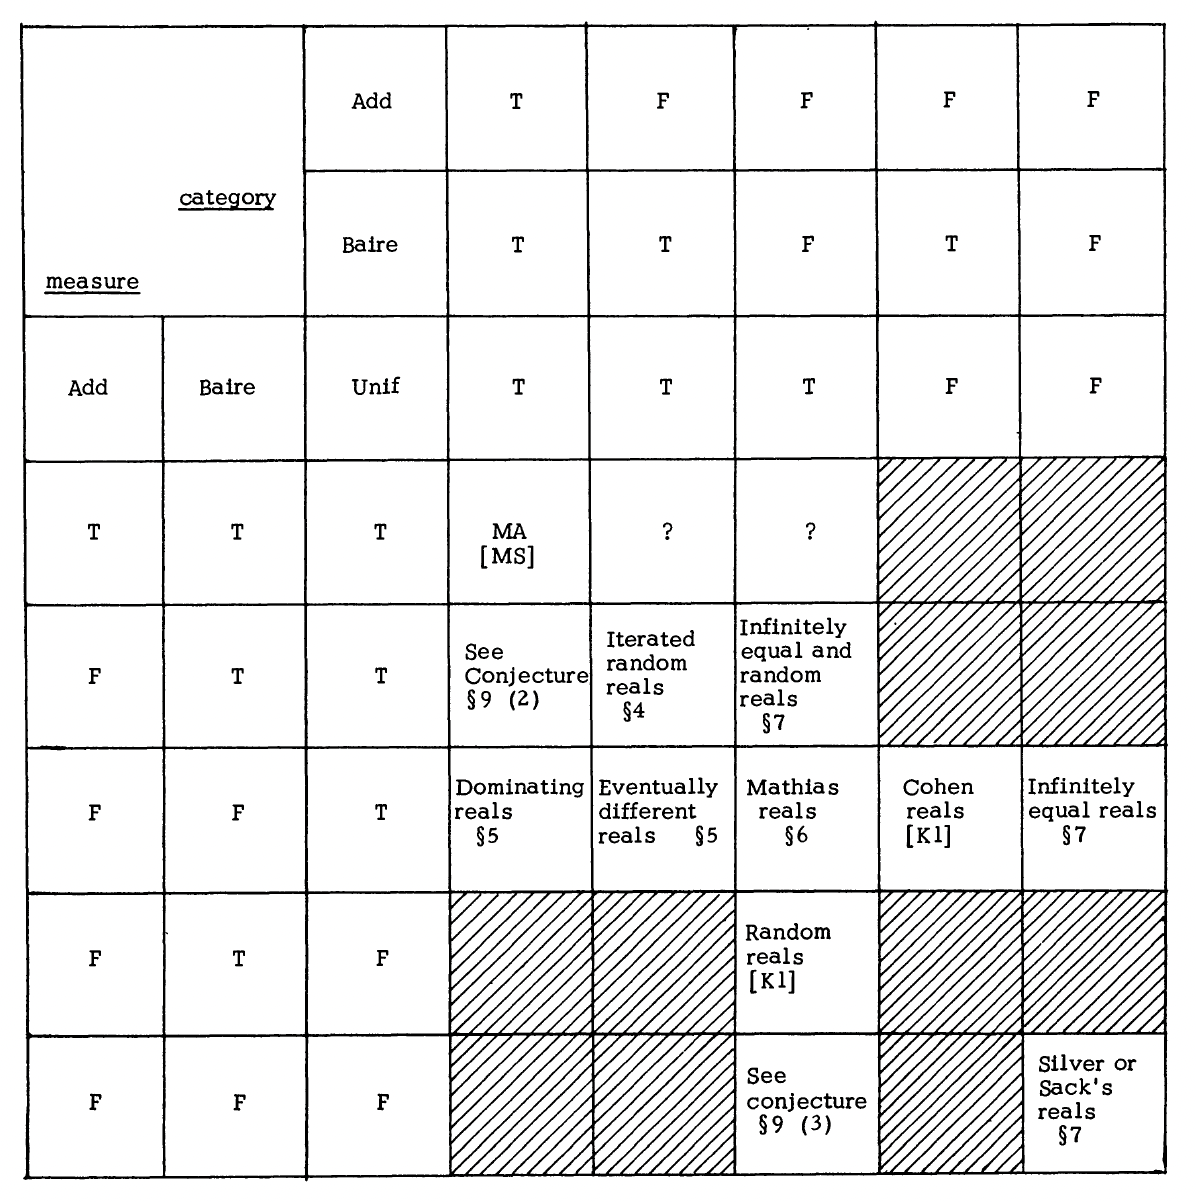
\includegraphics[width=7cm]{kunen-miller.png}
		\caption{Kunen-Millerの表}
		\end{center}
	\end{figure}
	
	表題にもなっているCichoń's maximumであるが,これはCichońの図式において (他の基数不変量の値に束縛されている$\add(\meager), \cof(\meager)$を除いて)すべての基数不変量の値を同時に別々の値にするモデルである.
	そのようなモデルの構成法を本稿では見ていく.
	
	\subsection{関係システム}
	
	\begin{defi}
		3つ組$\relR = (X, Y, \sqsubset)$が\textbf{関係システム}であるとは,$X, Y$が集合で$\sqsubset$が関係であることを言う (基本的には$\mathord{\sqsubset} \subset X \times Y$だがはみ出ていてよい).
		
		$F \subset X$が$\relR$\textbf{有界}であるとは$(\exists y \in Y)(\forall x \in F) (x \sqsubset y)$を満たすことである.
		$E \subset Y$が$\relR$\textbf{-dominanting}であるとは$(\forall x \in X)(\exists y \in E) (x \sqsubset y)$を満たすことである.
		
		\begin{itemize}
			\item $\frakb_\relR = \min \{ \abs{F} :  F \subset X \text{は}\relR\text{非有界} \}$
			\item $\frakd_\relR = \min \{ \abs{E} :  E \subset Y \text{は}\relR\text{-dominating} \}$
		\end{itemize}
		と定める.
	\end{defi}

	\begin{defi}
		関係システム$\relR = (X, Y, \sqsubset)$についてその双対を$\relR^\perp = (Y, X, \sqsubset^\perp)$と定める.ここに
		\[
		y \sqsubset^\perp x \iff \neg (x \sqsubset y).
		\]
	\end{defi}

	$\frakb_{\relR^\perp} = \frakd_\relR$かつ$\frakd_{\relR^\perp} = \frakb_\relR$に注意する.
	
	\begin{defi}
		関係システム$\relR = (X, Y, \sqsubset)$が\textbf{ポーランド関係システム}であるとは,次の3条件を満たすことを言う.
		\begin{enumerate}
			\item $X$は完全ポーランド空間.
			\item $Y$はあるポーランド空間$Z$の非空な解析集合.
			\item $\mathord{\sqsubset} \cap (X \times Z) = \bigcup_{n \in \omega} \mathord{\sqsubset}_n$であって,$\seq{\mathord{\sqsubset}_n : n \in \omega}$は$X \times Z$の閉集合の増大列であって,各$n \in \omega$と$y \in Y$について$(\mathord{\sqsubset}_n)^y = \{x \in X : x \sqsubset_n y \}$はnowhere denseである.
		\end{enumerate}
	\end{defi}

	ポーランド関係システムのような定義可能な関係システムを考えているとき,それを書いたときには今考えている宇宙の中でその定義を解釈したものを表すことにする.

	\begin{fact}
		$\relR$がポーランド関係システムであれば,$\frakb_\relR \le \non(\meager)$かつ$\cov(\meager) \le \frakd_\relR$である.
	\end{fact}

	\begin{defi}
		\begin{enumerate}
			\item $\mathcal{C} = \{ (q_n)_{n \in \omega}	 : \text{各}q_n\text{は正の有理数かつ} \sum_n q_n \le 1 \}$とおく.
			\item $\Omega_n = \{ a \in [2^{<\omega}]^{<\aleph_0} : \mu(\bigcup_{s \in a} [s]) \le 2^{-n} \}$とおき,$\Omega = \prod_{n \in \omega} \Omega_n$とおく.各$x \in \Omega$について$N_x = \bigcap_{n \in \omega} \bigcup_{s \in x(n)} [s]$とおく.
		\end{enumerate}
	\end{defi}

	以下の4つはすべてポーランド関係システムである.
	
	\begin{defi}
		\begin{enumerate}
			\item $\relR_1 = (\mathcal{C}, \mathcal{C}, \{(x,y) : (\forall^\infty n) (x(n) \le y(n))\})$
			\item $\relR_2 = (\Omega, 2^\omega, \{ (x, y) : y \not \in N_x \})$
			\item $\relR_3 = (\omega^\omega, \omega^\omega, \{ (x,y) : (\forall^\infty n)(x(n) \le y(n))\})$
			\item $\relR_4 = (\omega^\omega, \omega^\omega, \{ (x,y) : (\forall^\infty n)(x(n) \ne y(n)) \})$
		\end{enumerate}
	\end{defi}

	\begin{lem}
		\begin{enumerate}
			\item $\frakd_{\relR_1} = \cof(\nul), \frakb_{\relR_1} = \add(\nul)$,
			\item $\frakd_{\relR_2} = \non(\nul), \frakb_{\relR_2} = \cov(\nul)$,
			\item $\frakd_{\relR_3} = \frakd, \frakb_{\relR_3} = \frakb$,
			\item $\frakd_{\relR_4} = \cov(\meager), \frakb_{\relR_4} = \non(\meager)$.
		\end{enumerate}
	\end{lem}
	
	\subsection{Cohen,ランダム,Hechler,アメーバ,eventually different強制法}
	
		\subsubsection{Cohen強制法}
		
		$\C = 2^{<\omega}$で順序を延長関係で入れたもの$q \le p \iff p \subset q$はCohen強制法と呼ばれる.
		$\C$ジェネリックフィルター$G$から作られる実数$c = \bigcup G$をCohen実数という.
		Cohen実数から$G$を復元できる:$G = \{ c \upharpoonright n : n \in \omega \}$.
		Cohen強制法は可算なので,明らかに$\sigma$-centeredを満たす.特にcccを満たす.
		Cohen実数は$\relR_4^\perp$を解決する:
		\[
		(\forall x \in \omega^\omega \cap V)(\exists^\infty n)(x(n) = \dot{c}(n)).
		\]
		
		\subsubsection{ランダム強制法}
		
		$\B = \{ T : T\text{は}2^{<\omega}\text{の部分木で}\mu([T]) > 0 \}$で順序を包含関係で入れたもの$T' \le T \iff T' \subset T$をランダム強制法という.
		$\B$ジェネリックフィルター$G$から作られる実数$r = \bigcap \{[T] : T \in G \}$をランダム実数という.
		ランダム実数から$G$を復元できる:$G = \{ T \in \B : r \in [T] \}$.
		ランダム強制法はcccを満たす.
		ランダム実数は$\relR_2$を解決する:
		\[
		(\forall x \in \Omega^V)(\dot{r} \not \in N_x).
		\]
		
		\subsubsection{Hechler強制法}
		
		$\mathbb{D} = \{ (n, f) : n \in \omega, f \in \omega^\omega \}$で順序を
		\[(m, g) \le (n, f) \iff n \le m \land f \upharpoonright n = g \upharpoonright n \land (\forall k \in \omega)(f(k) \le g(k))\]
		で入れたものをHechler強制法という.
		$\mathbb{D}$ジェネリックフィルター$G$から作られる実数$d = \bigcup \{ f \upharpoonright n : (n, f) \in G \}$をHechler実数という.
		Hechler実数から$G$を復元できる:$G = \{ (n, f) : f \upharpoonright n = d \upharpoonright n \}$.
		Hechler強制法は$\sigma$-centeredである.
		Hechler実数は$\relR_3$を解決する:
		\[
		(\forall x \in \omega^\omega \cap V)(\forall^\infty n)(x \le^* \dot{d}).
		\]
		
		\subsubsection{アメーバ強制法}
		
		$\mathbb{A} = \{ T : T\text{は}2^{<\omega}\text{のsubtreeで}\mu([T])\ge 1/2 \}$で順序を$T' \le T \iff T' \subset T$で入れたものをアメーバ強制法という.
		$\mathbb{D}$ジェネリックフィルター$G$に対して測度$1/2$の閉集合$K_G = \bigcap G$が定まる.そのコード$a$をアメーバ実数という.アメーバ実数$a$から$G$を復元できる: $G = \{ T \in \mathbb{A} : \hat{a} \subset [T] \}$.
		アメーバ実数をBorelな方法で加工して得られる実数$b \in \mathcal{C}$があって,それは$\relR_1$を解決する:
		\[
		(\forall x \in \mathcal{C}^V) (x \le b).
		\]
		アメーバ強制法はcccである.
		
		\subsubsection{eventually different強制法}
		
		$\mathbb{E} = \{ (s,k,\varphi) : s \in \omega^{<\omega}, k \in \omega, \varphi \colon \omega \to [\omega]^{\le k}, (\forall i \in \dom(s))(s(i) \not \in \varphi(i)) \}$で順序を
		\[
		(s', k', \varphi') \le (s, k, \varphi) \iff s \subset s' \land k \le k' \land (\forall i)(\varphi(i) \subset \varphi'(i))
		\]
		を入れたものをeventually different強制法という.	
		$\mathbb{E}$ジェネリックフィルター$G$から作られる実数$e = \bigcup \{ s  : (s, k, \varphi) \in G \}$をeventually different generic実数という.
		eventually different強制法は$\sigma$-centeredである.
		eventually different generic実数は$\relR_4$を解決する:
		\[
		(\forall x \in \omega^\omega \cap V)(\forall^\infty n)(x(n) \ne \dot{e}(n)).
		\]
		
		\subsubsection{Borel reading of names}
		
		Cohen,ランダム,Hechler,アメーバ,eventually different強制法は共通して次の性質を持つ.
		
		\begin{property}\label{property:hasgenericreal}
			$\P$をcccかつBorelな強制半順序であり,かつ$\P$はジェネリック実数を持つという性質を考える.
			すなわち,実数の名前$\dot{x}_\mathrm{gen}$とBorelな関係$B \subset \P \times 2^\omega$があって
			\[
			\P \forces p \in \dot{G} \iff B(p, \dot{x}_\mathrm{gen})
			\]
			となるという性質を考える.
		\end{property}
	
		この性質を持つ強制法による強制拡大での実数はジェネリック実数からBorelな方法で計算できる.
		\begin{prop}
			$\P$を上記性質\ref{property:hasgenericreal}を持つ強制法とする.
			$\dot{x}$を$2^\omega$の元の名前とする.
			このときBorel関数$C \colon 2^\omega \to 2^\omega$があって,
			\[
			\forces \dot{x} = C(\dot{x}_\mathrm{gen})
			\]
			となる.
		\end{prop}
	
		これは有限台反復でも同様である.
		\begin{prop}
		$(P_\alpha, Q_\alpha : \alpha < \delta)$を有限台反復とする.
		各$Q_\alpha$は上記性質\ref{property:hasgenericreal}を持つ(ことが$P_\alpha$によって強制される)強制法とする.
		$\dot{x}$を$2^\omega$の元の$P_\delta$名前とする.
		このときBorel関数$C \colon (2^\omega)^\omega \to 2^\omega$と可算個の添字$\alpha_0, \alpha_1, \dots$があって,
		\[
		\forces \dot{x} = C(\dot{x}_\mathrm{gen}^{\alpha_0}, \dot{x}_\mathrm{gen}^{\alpha_1}, \dots)
		\]
		となる.
		\end{prop}
		
	\subsection{goodness}
	
	\begin{defi}
		$P$をcccな強制法とし,$\lambda$を非可算正則基数とし,$R$をポーランド関係システムとする.
		$P$が\textbf{$\lambda$-$\relR$-good}であるとは,$Y$の元を表す各$P$名前$\dot{y}$について非空な集合$\mathscr{Y} \subset Y$でサイズ$<\lambda$なものが$V$に存在して,どんな$x \in X$についても$x$が$\mathscr{Y}$上$\relR$非有界であれば,$\forces x \not \sqsubset \dot{y}$.
	\end{defi}

	\begin{fact}
		$\relR$をポーランド関係システムとする.
		\begin{enumerate}
			\item cccでサイズ$< \lambda$な強制法$P$はすべて,$\lambda$-$\relR$-goodである.特にCohen強制法は$\aleph_1$-$\relR$-goodである.
			\item cccで$\lambda$-$\relR$-goodであることは任意の長さの有限台反復で保たれる.
		\end{enumerate}
	\end{fact}

	\begin{fact}\label{fact:goodness}
	\begin{enumerate}
		\item $\sigma$-centeredかランダム強制法の部分ブール代数である強制法は$\aleph_1$-$\relR_1$-goodである.
		\item $\sigma$-centeredな強制法は$\aleph_1$-$\relR_2$-goodである.
	\end{enumerate}
	\end{fact}

	\begin{lem}\label{lem:cohenreals}
		$\relR = (X, Y, \sqsubset)$をポーランド関係システムとする.
		$\lambda \le \kappa \le \mu$を全て非可算正則基数とする.
		$\mu$個のCohen実数$(c_\alpha : \alpha < \mu)$を加えた後に,$\lambda$-$\relR$-good強制法で強制拡大したモデルにおいて,どんな実数$y \in Y$についても,
		\[
		(\exists \alpha < \kappa)(\forall \beta \in \kappa \setminus \alpha)(c_\beta \not \sqsubset y)
		\]
		が成り立つ.
	\end{lem}
	\begin{proof}
		$\kappa$個のCohen実数を追加した後の中間モデルで議論する.それを$V_\kappa$と呼ぶ.
		残りの強制法,すなわち$\mu\setminus\kappa$個のCohenとgood強制法の反復はgoodである.
		よって$V_\kappa$においてgoodnessを目撃する集合$\mathcal{Y}$でサイズ${<}\lambda$なものを得る. 

		最初のCohen強制法はcccであり,$\kappa\ge \lambda$は正則なので,ある番号$\alpha\in\kappa$がとれてどの元$y \in \mathcal{Y}$もすでに
		最初の$\alpha$個のCohenを付け加えたモデルに存在する.そのモデルを$V_{\alpha}$と書こう.
		$y$によってboundされる実数たちの集合$M_y$はmeagerであり,それは絶対的である.
		どの$\beta\in\kappa\setminus \alpha$に対しても$c_\beta$は$V_{\alpha}$上のCohen実数なので$M_y$に属さない.すなわち$y$にboundされない.
		つまり,$\mathcal Y$によってboundされない.
		したがって,goodnessの定義より,各$c_\beta$は与えられた$y$にboundされないことが強制される.
	\end{proof}
	
	\subsection{$\EUB$と$\COB$}
	
	\begin{defi}
		$\gamma$を極限順序数,$P$をccc強制法,$\relR = (X, Y, \sqsubset)$を定義可能な関係システムとする.
		$\EUB(\relR, P, \gamma)$とは次の主張である:
		$X$の元の$P$-名前の列$(\dot{x}_\alpha)_{\alpha < \gamma}$であって,どんな$Y$の元の$P$-名前の列$\dot{y}$についても
		\[
		(\exists \alpha < \gamma)(\forall \beta \in \gamma \setminus \alpha)\ P \forces \neg (\dot{x}_\beta \sqsubset \dot{y})
		\]
		となる.
	\end{defi}
	ccc強制法を考えているので,$\gamma$が非可算共終数を持つときには,$(\exists \alpha < \gamma)(\forall \beta \in \gamma \setminus \alpha)$は強制関係の外にあろうが中にあろうが同じなことに注意しておく.
	
	\begin{defi}
		$\lambda, \mu$を非可算正則基数,$P$をccc強制法,$\relR = (X, Y, \sqsubset)$を定義可能な関係システムとする.
		このとき$\COB(\relR, P, \lambda, \mu)$は次の主張である:
		${<}\lambda$-directedな半順序集合集合$(S, \prec)$でサイズ$\mu$なものと$Y$の元の$P$-名前の族$(\dot{y}_s : s \in S)$があって,$X$の元のどんな$P$-名前$\dot{x}$についても
		\[
		(\exists s \in S)(\forall t \succ s) \ P \forces \dot{x} \sqsubset \dot{y}_i
		\]
		となる.
	\end{defi}

	$\EUB(\relR, P, \gamma)$は$\COB(\relR^\perp, P, \cf(\gamma), \cf(\gamma))$と同値なことに注意する.
	
	\begin{lem}\label{lem:cobimpliesineq}
		$\COB(\relR, P, \lambda, \mu)$は$P \forces (\frakb_\relR \ge \lambda \AND \frakd_\relR \le \mu)$を含意する.
		また$\EUB(\relR, P, \lambda)$は$P \forces (\frakb_\relR \le \lambda \AND \frakd_\relR \ge \lambda)$を含意する.
	\end{lem}
	\begin{proof}
		前半の$\COB$についての主張の証明.
		集合$(\dot{y}_s)_{s\in S}$はサイズ$\mu$のdominating familyなので$\mathfrak{d}_\relR\le \mu$を得る.

		$\mathfrak{b}_\relR \ge \lambda$を示すために,$(\dot{x}_\alpha)_{\alpha\in\theta}$を長さ$\theta<\lambda$なる$X$の元の$P$名前の列とする.
		各$\dot{x}_\alpha$について,$s_\alpha\in S$があって,$(\forall t\succ s_\alpha)\, P\forces \dot{x}_\alpha \sqsubset \dot{y}_t$である.
		$S$は${<}\lambda$-directedなので,ある$t$があってどの$s_\alpha$よりも大きい.
		したがって,$P\forces \dot{x}_\alpha \sqsubset \dot{y}_t $がすべての$\alpha$で成り立つ.
		すなわち$\{\dot{x}_\alpha:\, \alpha\in\theta\}$はboundedである.
		
		後半の$\EUB$についての主張は上の主張と前半の主張から従う.
	\end{proof}

	\section{Cichońの図式の左半分}\label{sec:leftside}
	
	\subsection{初めの強制法$\Pa$}

	これから「部分的アメーバ強制法」「部分的ランダム強制法」「部分的Hechler強制法」「部分的eventually different強制法」を定義する.
	そのために,性質\ref{property:hasgenericreal}を持つ強制法の有限台反復$(P_\alpha, Q_\alpha : \alpha < \delta)$を考える.
	$(\dot{\eta}_\alpha : \alpha < \delta)$をジェネリック実数の列とする.
	$\alpha < \delta$と$w \subset \alpha$を固定する.

	\begin{defi}
		\begin{enumerate}
		\item $V$の元$(B, u)$が\textbf{$w$-コード}であるとは,$u$が$u \subset w$なる可算集合であり$B$が$B \colon \R^u \to \R$なるBorel関数であることを意味する.
		\item $V^{P_\alpha}$の実数$x$が$w$-コード$(B, u)$の\textbf{解釈}であるとは,$x = B((\eta_\beta)_{\beta \in u})$であることを意味する
		\item $\dot{Q}_\alpha$が\textbf{$w$-部分的ランダム強制法}であるとは,
		\[
			P_\alpha \forces Q_\alpha = \{ q : q \text{はランダム強制法の条件であり,}q\text{はある}w\text{-コード}(B, u)\text{ in }V\text{の解釈}\}	
		\]
		となっていることを意味する.ただし,$Q_\alpha$の順序はランダム強制法の順序の制限であるとする.
		\end{enumerate}
	\end{defi}

	ランダム強制法以外のアメーバ・Hechler・eventually different強制法についても$w$-部分的強制法を同様に定義する.
	
	\begin{assumption}\label{asm:P}
		$\aleph_1<\lambda_1<\lambda_2<\lambda_3<\lambda_4<\lambda_5$を正則基数たちで
		$\mu<\lambda_i$ならば$\mu^{\aleph_0}<\lambda_i$となるものたちとする.
		また,$\lambda_3$は正則基数$\chi$で$\chi^{\aleph_0}=\chi$なものの後続基数だと仮定し,$\lambda_5^{<\lambda_4}=\lambda_5$とする.
		
		$\delta_5=\lambda_5+\lambda_5$とおき,$\delta_5\setminus\lambda_5$の非有界部分集合たち$S^1$, $S^2$, $S^3$ and $S^4$への分割を固定する.
		各$\alpha\in \delta_5\setminus\lambda_5$ について$w_\alpha\subseteq \alpha$であって各$\{w_\alpha:\, \alpha\in S^i\}$は $[\delta_5]^{{<}\lambda_i}$の中で共終であると仮定する.
	\end{assumption}
	
	\begin{defi}\label{def:Pa}
		$\Pa=(P_\alpha,Q_\alpha)_{\alpha\in\delta_5}$ 
		を有限台反復であって,$\alpha\in \lambda_5$に対する$Q_\alpha$はCohen強制法であり
		\begin{flalign*}
			&&
			Q_\alpha\text{ は$w_\alpha$-部分的 }
			\left\{
			\begin{array}{c}
				\text{アメーバ}\\
				\text{ランダム}\\
				\text{Hechler}\\
				\text{eventually different}\\
			\end{array}\right\}
			\text{ 強制法} \hspace{0.5cm} \text{($\alpha$が}
			\left\{
			\begin{array}{l}
				S^1\\
				S^2\\
				S^3\\
				S^4\\
			\end{array}
			\right\} \text{の元のとき)}
			\\
		\end{flalign*}
		であるものとする.
	\end{defi}

	事実 \ref{fact:goodness}より$\Pa$は$i\in\{1,2,4\}$について$(\lambda_i, \relR_i)$-goodである.
	したがって補題 \ref{lem:cohenreals}より次が従う.

	\begin{lem}
		$i \in \{1,2,4\}$と正則基数$\kappa \in [\lambda_i, \lambda_5]$について$\EUB(\relR, \Pa, \kappa)$が成り立つ.
	\end{lem}

	\begin{lem}
		$i \in \{1,2,3,4\}$について$\COB(\relR, \Pa, \lambda_i, \lambda_5)$が成り立つ.
	\end{lem}
	\begin{proof}
		$S=S^i$とおき,$S$上の順序$\prec$を$s\prec t \iff w_s\subsetneq w_t$で定める.
		$\lambda_i$が正則なので$(S,\prec)$は${<}\lambda_i$-directedである.
		$\dot{y}_s$を$s$で追加されるジェネリック実数とする (たとえば,$i=2$のときは部分的ランダム実数).
		$\Pa$名前$\dot{x}$はBorelな方法で 
		ジェネリック実数たちの可算な添字の集合$w^*\subseteq \delta$による部分列のみに依存する.
		$s\in S^i$であって$w_s\supseteq w^*$となるものをとる.
		$t\succ s$を任意にとる.
		このとき$w_t\supseteq w_s$なので$w_t$は$\dot{x}$を計算するためのすべての情報を含む.
		よって,$\Pa \forces \dot{x} \sqsubset_i \dot{y}_t$を得る.
	\end{proof}
	
	\subsection{$\frakb$を$\GCH$なしで取り扱う}
	
	前の節の内容では$\EUB(\relR_3, \Pa, \kappa)$ (これは$\frakb$が小さいことに対応する)が抜けていたことに注意しよう.
	適切にパラメータ$(w_\alpha)_{\alpha \in S^4}$を選ぶことでこの$\EUB$も得られることをこの節と次の節で見ていく.
	
	この節に限って,仮定 \ref{asm:P}に加えて次も仮定する.
	
	\begin{assumption}\label{asm:chi}
		(この節限定) $2^\chi =|\delta_5|= \lambda_5$.
	\end{assumption}
	
	$S^0=\lambda_5\cup S^1\cup S^2\cup S^3$とおく.
	よって$\delta_5=S^0\cup S^4$であり,$\Pa$ は長さ$\delta_5$のFS ccc反復であり,$\alpha\in S^0$は$\abs{Q_\alpha}<\lambda_3$を含意する.すなわち$\abs{Q_\alpha}\le\chi$を含意する.
	$\alpha \in S^0$に対して$P_\alpha$名前
	\begin{equation}\label{eq:ia}
		i_\alpha:Q_\alpha\to\chi\text{ 単射}
	\end{equation}
	を固定する.
	
	各条件$p\in \Pa$はある条件$q$に強めて$\alpha\in \supp(q)\cap S^0$ならば $q\restriction\alpha\forces i_\alpha(q(\alpha))=\check \jmath$ for some 
	$j\in\chi$となるようにできることに注意しておく.
	
	eventually different強制法について再掲しておく.
	$\mathbb{E} = \{ (s,k,\varphi) : s \in \omega^{<\omega}, k \in \omega, \varphi \colon \omega \to [\omega]^{\le k}, (\forall i \in \dom(s))(s(i) \not \in \varphi(i)) \}$で順序を
	\[
	(s', k', \varphi') \le (s, k, \varphi) \iff s \subset s' \land k \le k' \land (\forall i)(\varphi(i) \subset \varphi'(i))
	\]
	を入れたものをeventually different強制法という.	
	$\mathbb{E}$ジェネリックフィルター$G$から作られる実数$e = \bigcup \{ s  : (s, k, \varphi) \in G \}$をeventually different generic実数という.
	$(s, k, \varphi) \in \mathbb{E}$に対して$s$を\textbf{幹},$k$を\textbf{幅}と呼ぶことにする.
	
	次の性質たちは容易に観察できる.
	\begin{observation}
	\begin{itemize}
		\item \label{compat.a} もし$p,q\in \Eor$が両立可能ならばそれらは最大の共通下界を持つ. 
		\item \label{compat.b} 同じ幹を持つ有限個の条件について,それらは同じ幹の共通下界を持つ.よって,$\Eor$は$\sigma$-centeredである.
		\item もし$q=(s',k',\varphi')$かつ$p=(s,k,\varphi)$であって$s'$が$s$の延長であるならば,$p$と$q$が両立可能であるのは,ちょうど
		$s'(i)\notin \varphi(i)$ for all $i\in\dom(s')$であるときである.
		\item  \label{compat.c}  もし$q^* =(s^*,k^*,\varphi^ *)$が有限集合$B\subseteq \Eor$のすべての元と両立可能ならばかつ$s^*$が各$(s,k,\varphi)\in B$について$s$の延長ならば,$B\cup \{q^*\}$は下界を持つ. 
		($s^*$を幹として使い,$B\cup \{q^ *\}$に現れるすべての$\varphi$のpointwiseの和集合をとればよい.)
	\end{itemize}
	\end{observation}

	我々は$\Eor$ではなく$\Eor$の部分的バージョンで強制する.
	$\alpha \in S^4$に対する$P_\alpha$拡大において,この部分強制$Q_\alpha=\Eor'$は
	(必ずしも完備埋め込みでない)$\Eor$の部分強制法であり,conjunctionで閉じている
	(すなわち,条件の有限集合について最大下界を取る部分操作で閉じている).
	よって両立可能性は$\Eor$で見ても$\Eor'$で見ても変わらない.
	そして先程の観察は$\Eor'$に対しても成り立つ.後の参照のために最後の項目を明示的に主張しておく.
	
	
	\begin{fact}\label{fact:bla}
		$\Eor'\subseteq \Eor$がconjuctionで閉じているものとする.
		もし条件$q^* =(s^*,k^*,\varphi^ *) \in \Eor'$が有限集合$B\subseteq \Eor'$のどの元とも両立可能かつ$s^*$が各$(s,k,\varphi)\in B$に対する$s$の延長ならば$B\cup \{q^*\}$は下界を$\Eor'$に持つ. 
	\end{fact}


	\begin{defi}
		$D$を$\omega$上の非単項ウルトラフィルターとし$\bar p = 
		(p_n)_{n\in \omega} = (s,k,\varphi_n)_{n\in \omega}$を$\Eor$の条件の列であって,同じ幹と幅を持つものとする. 
		$\lim_D\bar p$という条件を$(s,k,\varphi_\infty)$であって,すべての$i$と$j$について
		$
		j\in \varphi_\infty(i) \Leftrightarrow \{ n: j\in \varphi_n(i)\}\in D
		$.
		となるものとして定める.
	\end{defi}

	$\lim_D\bar p\in\Eor$である.また,$q\le \lim_D \bar p$ならば集合$B\coloneq\{ n\in \omega:\, p_n \text{ compatible with } q\}$は$D$の元である.
	
	(証明: $q=(s',k',\varphi')\le \lim_D\bar p=(s,k,\varphi_\infty)$とする.よって各$i\in\dom(s')$について$s'(i)\notin \varphi_\infty(i)$であり,極限の定義より$A^i \coloneq\{n:\, s'(i)\notin \varphi_n(i)\}\in D$である.もし$n\in\bigcap_{i\in\dom(s')} A^i$ならば$p_n$は$q$と両立する.)
	
	
	集合$B$は両立可能性のみを使って定義されているので,両立可能性を保存する部分強制に対してなお主張は成り立つ.
	後の参照のためにこれを述べておく:
	\begin{fact}\label{fact:blubb4}
		$\Eor'$がconjunctionで閉じた$\Eor$の部分強制で$\bar p$が$\Eor'$の条件の列で同じ幹と幅を持つものとし,$\lim_D(\bar p)\in \Eor'$と$q\le_{\Eor'} \lim_D(\bar p)$を仮定する.
		このとき
		$B\coloneq\{ n\in \omega:\, p_n \text{ compatible with } q\}$は$D$の元である.
	\end{fact}
		
		\begin{defi}
			\begin{itemize}
				\item \textbf{部分的なガードレール}とは関数$h$でその定義域は$\delta_5$の部分集合であり,$\alpha\in S^0\cap\dom(h)$について$h(\alpha)\in \chi$でかつ,$\alpha\in S^4\cap\dom(h)$について$h(\alpha)
				\in \omega^{<\omega}\times \omega$であるものである.
				\item \textbf{可算なガードレール}とは部分的なガードレールであって可算な定義域を持つものである.
				\textbf{フルガードレール}とは部分的ガードレールで定義域が$\delta_5$なものである.
			\end{itemize}
		\end{defi}
	
	EngelkingとKar{\l}owicz \cite{engelking1965some}は位相空間のボックス積のdensityを調べるために次の補題を証明した.我々はこの結果を使う.
	
	\begin{lem}\label{lem:ek}
		$\theta, \mu$を無限基数とし$\mu^{<\theta} = \mu$とする.
		このとき,関数の族$(f_\xi : \xi < \mu)$であって各$f_\xi \colon 2^\mu \to \mu$であって,
		どんな関数$f$であって$\dom(f) \in [2^\mu]^{<\theta}$かつ$\range(f) \subset \mu$なものについてもある$\xi < \mu$があって$f \subset f_\xi$である.
	\end{lem}

	補題\ref{lem:ek}より次が従う.

	\begin{lem}\label{use.EK}
		($|\delta_5|\le 2^\chi$ and $\chi^{\aleph_0}=\chi$なので,)フルガードレールの族$H^*$で$|H^*|=\chi$なものがあり,各可算ガードレールはある$h\in H^*$に拡大される. 
		このような族$H^*$を一つ固定し,$(h^*_\ve)_{\ve\in \chi}$と$H^*$の元を枚挙する.
	\end{lem}

	\begin{defi}
		条件$p\in \Pa$がフルガードレール$h$に従うとは次の2条件を満たすことをいう.
		\begin{itemize}
			\item 
			すべての$\alpha\in S^0 \cap \dom(p)$について$P_\alpha$は$p(\alpha)\in Q_\alpha$かつ$i_\alpha(p(\alpha)) = h(\alpha)$を強制する ($i_\alpha$は\eqref{eq:ia}で定義されたもの)
			\item  すべての$\alpha\in S^4\cap \dom(p)$について:
			\begin{itemize}
				\item  $p\on\alpha$は$p(\alpha)$の幹と幅の組が$h(\alpha)$に等しいことを強制する.
				\item $p \on (\alpha+1)$は$\alpha$において決定されている.
			\end{itemize}
		\end{itemize}       
	\end{defi}
		
	\subsection{$\GCH$を復活させる}
	
	
	\begin{thm}\label{thm:Pa}
		GCHを仮定し$\lambda_i$が仮定\ref{asm:P}を満たすものとして与えられるとする.
		このときパラメータを適切に定めることで,定義\ref{def:Pa}でのFS ccc反復$\Pa$が$i=1,2,3,4$について次を満たすようにできる:
		\begin{itemize} 
			\item  任意の$[\lambda_i,\lambda_5]$内の正則基数$\kappa$について,$\EUB(\relR_i, \Pa,\kappa)$が成り立つ.
			\item $\COB(\relR_i, \Pa,\lambda_i,\lambda_5)$が成り立つ.
		\end{itemize}
		よって特に$\Pa$は$\addnull=\lambda_1$, $\covnull=\lambda_2$, 
		$\mathfrak{b}=\lambda_3$, $\nonmeager=\lambda_4$,
		$\covmeager=\mathfrak{d}=\nonnull=\cofnull=\lambda_5=2^{\aleph_0}$を強制する.
	\end{thm}
	
	\section{ブール超冪}
	
	\subsection{ブール超冪}
	
	$\kappa$を強コンパクト基数とし,$B$を$\kappa$分配的かつ$\kappa^+$-ccを持つ無原子完備ブール代数とする.
	すると任意の$B$内の$\kappa$完備フィルターは$\kappa$完備なウルトラフィルターに拡大される.
	$U$は$\kappa^+$完備ではない.
	%また,ある$B$の反鎖$A_0$で濃度$\kappa$なものがあって,$A_0 \cap U = \emptyset$を満たす.
	今,$\kappa$完備なウルトラフィルター$U$を固定する.
	
	\textbf{BUP名前}とは関数$x \colon A \to V$であって,その定義域$A$は$B$の極大反鎖であるものである.
	$x$の定義域を$A(x)$と書く.
	
	任意のBUP名前は$V$の元の$B$-名前を定める:BUP名前$x$に対して$\{ (\widecheck{x(a)}, a) : a \in A(x) \}$である.
	逆に$V$の元の$B$-名前はそれと強制同値なBUP名前を持つ.
	BUP名前とそこから定まる$B$-名前を同一視する.
	
	2つのBUP名前に対してブール値$\truth{x=y}$が定まる.$x$と$y$が同値とは$\truth{x=y} \in U$であることを指す.
	
	$v \in V$の標準名前$\check{v}$とは$\{ (1_B, w) : w \in v \}$のことである.
	
	ブール超冪$M^-$はBUP名前$x$の同値類$[x]$からなる.
	$[x] \in^- [y]$を$\truth{x \in y} \in U$により定義する.
	$j^- \colon V \to M^-$を$v$を$[\check{v}]$に送る写像として定める.
	
	BUP名前$x_1, \dots, x_n$に対してブール値$\truth{\varphi(x_1, \dots, x_n)}$が適切に定まる.

	次が成り立つ.
	\begin{enumerate}
		\item Łośの定理: $(M^-, \in^-) \models \varphi([x_1], \dots, [x_n])$が成り立つのはちょうど$\truth{\varphi(x_1, \dots, x_n)} \in U$のとき.
		\item $j^- \colon (V, \in) \to (M^-, \in^-)$は初等埋め込み.
		\item 特に$(M^-, \in^-)$は$\ZFC$のモデル.
	\end{enumerate}
	
	$U$が$\sigma$完備なので,$(M^-, \in^-)$はwellfoundedである.
	$M$を$(M^-, \in^-)$の推移崩壊とする.
	そして$j \colon V \to M$を$j^-$と推移崩壊写像の合成とする.
	$[x]$の推移崩壊$x^U$と書く.したがって,$\check{v}^U = j(v)$である.

	\begin{fact}
	\begin{enumerate}
		\item $M \models \varphi(x_1^U, \dots, x_n^U)$となるのはちょうど$\truth{\varphi(x_1, \dots, x_n)} \in U$となるとき.
		特に$j \colon V \to M$は初等埋め込み.
		\item $\abs{Y} < \kappa$ならば$j(Y) = j''Y$である.特に$j$の$\kappa$への制限は恒等写像である.$M$は${<}\kappa$列で閉じている.
		\item $j(\kappa) \ne \kappa$,特に$\kappa = \crit(j)$.
	\end{enumerate}
	\end{fact}
	\begin{proof}
		一つだけ示してみよう.$\alpha < \kappa$について$j(\alpha) = \alpha$を示す.
		背理法で,$j(\alpha) > \alpha$となる$\alpha$が存在するとして,そのような最小を取る.
		$\alpha \in j(\alpha) \in M$で$M$は推移的なので$\alpha \in M$である.
		そこでBUP名前$x$をとって$j(x) = \alpha$となる.
		$j(x) \in j(\alpha)$だからŁośの定理より$\truth{\check{x} \in \check{\alpha}} \in U$となる.
		今ブール値$\truth{\check{x} \in \check{\alpha}}$は$\bigvee_{\beta \in \alpha} \truth{\check{x} = \check{\beta}}$に等しいことと,$U$の$\kappa$完備性より,ある$\beta < \alpha$があって,$\truth{\check{x} = \check{\beta}} \in U$となる.
		Łośの定理をもう一度使うと$j(\beta) = j(x) = \alpha$.今$\beta$の最小性より$j(\beta) = \beta$だから$\beta = j(\beta) = j(x) = \alpha$となって,$\beta < \alpha$に反する.
	\end{proof}

	$V$の元$Y$について,$Y$の元を表す強制名前はBUP名前$x$でその値域$\range(x)$が$Y$の部分集合であるものとして書ける.
	そのようなBUP名前を\textbf{$j(Y)$の元を表すBUP名前}と呼ぶことにする (そのような名前$x$について$x^U$は$j(Y)$の元であるため).

	\begin{lem}
		$(S, \le)$を${\le} \kappa$-directedな半順序集合としたとき,$j''S$は$j(S)$の中でcofinalである.
	\end{lem}
	\begin{proof}
		$j(S)$の元を任意にとり,$x^U$とする.
		先程の注意より,BUP名前$x$は$\range(x) \subset S$としてよい.
		$\dom(x)$は$B$が$\kappa^+$-ccなことよりサイズ$\kappa$以下なので,$\range(x)$は共通の上界$s_0$を持つ.
		すると$\truth{x \le s_0} = 1_B$となるので,$(M^-, \in^-) \models [x] \le \check{s_0}$.
		したがって,$x^U \le j(s_0)$となる.
	\end{proof}

	\begin{defi}
		\textbf{BUP埋め込み}とは,初等埋め込み$j \colon V \to M$ ($M$は推移的)であって,臨界点$\kappa$を持つものであって,
		$M$は${<}\kappa$-closedかつ,どんな${\le}\kappa$-directedな半順序集合$S$についても$j''S$は$j(S)$内でcofinalになるものである.
	\end{defi}

	よって,$\kappa$-分配的かつ$\kappa^+$-cc原子なし完備ブール代数と$\kappa$完備ウルトラフィルターに対する上で定義した埋め込みはBUP埋め込みである.

	\begin{lem}
		$j$をBUP埋め込みで$\crit(j) = \kappa$なものとする.
		\begin{enumerate}
			\item $\abs{A} < \kappa$ならば,$j''A = j(A)$である.
			\item ある正則基数$\lambda < \kappa$について$S$が${<}\lambda$-directedな半順序であるとき,$j(S)$は${<}\lambda$-directedである.
			\item $\cf(\alpha) \ne \kappa$なる極限順序数$\alpha$について,$j''\alpha$は$j(\alpha)$の中で共終.よって特に$\cf(j(\alpha)) = \cf(\alpha)$.
		\end{enumerate}
	\end{lem}
	\begin{proof}
		1つ目.$f \colon \lambda \to A$全単射と$\lambda < \kappa$をとる.
		すると$M$で$j(f) \colon \lambda \to j(A)$ 全単射が成り立つ.
		よって,$x \in j(A)$とすると$\alpha < \lambda$がとれて$x = j(f)(\alpha)$だが,$j(f)(\alpha) = j(f(\alpha))$なので,これで良い.

		2つ目.$M$で$j(S)$は${<}\lambda$-directedな半順序なことが成り立ち,$M$が${<}\kappa$-closedなことを使うとよい.

		3つ目.$\cf(\alpha) = \lambda \ne \kappa$とする.
		$f \colon \lambda \to \alpha$を共終単調増加関数とする.
		$\lambda < \kappa$ならば$M$の中で$j(f) \colon \lambda \to j(\alpha)$が共終単調増加関数となるが,これは絶対的である.
		$\lambda > \kappa$ならば$\alpha$は${\le}\kappa$-directedな半順序なので,$j''\alpha$は$j(\alpha)$の中で共終である.
		よって$j''f = (j(\xi), j(f(\xi)))_{\xi < \lambda}$は$\cf(j'' \lambda) = \cf(j '' \alpha) = \cf(j(\alpha))$を目撃する.
		他方で,$\cf(j''\lambda) = \cf(\lambda) = \lambda$である.これで示せた.
	\end{proof}

	\subsection{$\kappa$から$\theta$へのBUP埋め込み}

	\begin{lem}
		$\kappa$を強コンパクト基数,$\theta > \kappa$を$\cf(\theta) > \kappa$なる基数とする.
		このときBUP埋め込み$j$で$\crit(j) = \kappa$かつ次の3条件を満たすものが存在する:
		\begin{enumerate}
			\item $\cf(j(\kappa)) = \cf(\theta)$かつ$j(\kappa) \ge \theta$.
			\item すべての$\mu$について$\abs{j(\mu)} \le \max(\mu, \theta)^\kappa$.
			\item 特に$\theta^\kappa = \theta$かつ$\kappa \le \mu \le \theta$ならば$\abs{j(\mu)} = \theta$.
		\end{enumerate}
	\end{lem}
	\begin{proof}
		次で定まる強制法$(P_{\kappa,\theta}, \supseteq)$の完備化を$B$とする:
		\[
			P_{\kappa,\theta} = \{ f : f\text{は}\theta\text{から}\kappa\text{への部分関数で濃度が}{<}\kappa\text{なもの} \}
		\]
		$B$は${<}\kappa$分配的かつ$\kappa^+$-ccを持つ.
		この強制法はジェネリックな関数$f^* \colon \theta \to \kappa$を付け加える.
		よって,各$\delta < \theta$に対して$f^*(\delta)$は$\kappa$の元を表す強制名前であり,したがってBUP名前である.

		1番について.
		$x$を$j(\kappa)$の元を表すBUP名前とする.
		すなわち$x$の定義域$A$は$B$の極大反鎖であり,値域は$\kappa$の部分集合である.
		$P_{\kappa,\theta}$が$B$で稠密なので,$A \subset P_{\kappa,\theta}$と仮定してもよい.
		$\delta < \theta$を各$a \in A$について$a$の定義域の上限より大きいものとする($\cf(\theta) > \kappa$よりこれはある).
		このような$(x, \delta)$を「適切な組」と呼ぶことにする.
		そして
		\[
		b_{x,\delta} = \truth{ f^*(\delta) > x }	
		\]
		とおく.

		今,$b_{x,\delta}$たちが$\kappa$完備なフィルターを生成することを主張する.
		それを示すために,$(x_i, \delta_i : i < \mu)$, $\mu < \kappa$を適切な組の列とする.
		$\bigwedge_{i < \mu} b_{x_i, \delta_i} \ne \emptyset$を示す必要がある.
		集合$\{\delta_i : i < \mu\}$の元を単調増加かつ重複なしに$(\delta^\ell : \ell < \gamma)$, $\gamma \le \mu$と並べる.
		$A_\ell = \{ i < \mu : \delta_i = \delta^l \}$とおく.
		条件$q_\ell$が与えられたときに$q_{\ell+1} \in P_{\kappa, \theta}$を次のように定める:
		\begin{enumerate}
			\item $q_{\ell+1} \le q_{\ell}$
			\item $\delta^\ell \in \supp(q_{\ell+1}) \subset \delta^\ell \cup \{\delta^\ell \}$
			\item $q_{\ell+1} \upharpoonright \delta^\ell$はすべての$i < A^\ell$について$x_i$の値を$\alpha_i$に決定する.
			\item $q^{\ell+1}(\delta^\ell) = \sup_{i\in A_\ell}(\alpha_i)+1$
		\end{enumerate}
		この構成は$q_{\ell+1}$が各$i \in A_\ell$について$b_{x_i, \delta_i}$より強いことを保証する.
		極限順序数$\ell \le \gamma$についてはそこまで構成した条件の和集合をとる.
		すると$q_\gamma$は各$b_{x_i, \delta_i}$より強い条件となり主張が証明された.

		さて,$\kappa$が強コンパクトなので,$b_{x, \delta}$ ($(x, \delta)$は適切な組)が生成する$\kappa$完備フィルターを拡大して,$\kappa$完備ウルトラフィルター$U$を得ることができる.
		すると列$(f^*(\delta)^U : \delta < \theta)$は狭義単調増加かつ共終である ($\delta < \delta'$に対して$(f^*(\delta), \delta')$は適切であり,適切な組の$b$は$U$に入れていることから).
		よって,$\cf(j(\kappa)) = \cf(\theta)$かつ$j(\kappa) \ge \theta$を得る.

		2番について.
		$j(\mu)$の元を表すBUP名前の数を勘定すればよい.
		反鎖は$P_{\kappa,\theta}$の部分集合としてよかったので,$\abs{P_{\kappa,\theta}} = \theta$を考えると,$j(\mu)$の元を表すBUP名前の数は
		\[
			[\theta]^\kappa \times \mu^\kappa = \max(\theta, \mu)^\kappa
		\]
		で抑えられる.したがって,
		\[
		\abs{j(\mu)} \le \max(\theta, \mu)^\kappa.
		\]
	\end{proof}

	\begin{defi}
		\textbf{$\kappa$から$\theta$へのBUP埋め込み}とはBUP埋め込み$j$で臨界点$\kappa$を持ち,$\cf(j(\kappa)) = \abs{j(\kappa)} = \theta$となるものを言う.
	\end{defi}

	\begin{cor}\label{cor:embed}
		$\kappa$を強コンパクト,$\theta > \kappa$を正則基数で$\theta^\kappa = \theta$とする.
		すると$\kappa$から$\theta$へのBUP埋め込みが存在する.(なおかつそれは,$\kappa \le \mu \le \theta$なる$\mu$に対して$\abs{j(\mu)} = \theta$を満たす).
	\end{cor}

	\begin{lem}\label{lem:aa}
		$j \colon V \to M$を初等的で,$M$は推移的かつ${<}\kappa$-closedかつ$\crit(j) = \kappa$だとする.
		ある$\nu < \kappa$について$P$は$\nu$-ccであると仮定する.
		\begin{enumerate}
			\item\label{item:aa1} $j(P)$は$\nu$-cc.
			\item\label{item:aa2} $\tau$が$M[G]$の元を表す$j(P)$名前ならば,$j(P)$名前が$\sigma$が$M$の中にあって$j(P) \forces \tau=\sigma$となる.
			\item\label{item:aa2b}
			特に,どんな$j(P)$名前であって,実数やボレルコード,実数の可算列を表すものは同値なものが$M$の中にある.
			\item\label{item:aa3}  $M[G]$は$V[G]$の中で${<}\kappa$-closedである.
			\item\label{item:size} もし$\xi<\kappa$であって$P$が$2^\xi=\lambda$を強制するならば$j(P)$は$2^\xi=|j(\lambda)|$を強制する.
			\item\label{item:aa4} 
			$j''P$ (これは$P$と同型)は$j(P)$の完備部分強制法である.
		\end{enumerate}
	\end{lem}
	\begin{proof}
		1番について.
		$P$が$\nu$-ccなため,
		\[
		V \models \forall A \in [P]^\nu \exists p, q \in A (p \ne q \land p \parallel q)
		\]
		となる.初等性と$j(\nu) = \nu$より
		\[
		M \models \forall A \in [j(P)]^\nu \exists p, q \in A (p \ne q \land p \parallel q).
		\]
		$A \subset j(P)$がサイズ$\nu$だとしたら,$M$の${<}\kappa$closedより,$A \in M$である.
		そこで$M$で$\exists p, q \in A (p \ne q \land p \parallel q)$が成り立つが,これは上向き絶対的であるため, $V$でも成り立つ.
				
		2番について.

		\todo
	\end{proof}

	\subsection{$\EUB$と$\COB$の保存}

	\begin{lem}
		$\relR$をポーランド関係システムとし,$P$をccc強制法とし,$j$をBUP埋め込みで臨界点$\kappa$を持つものとする.
		このとき,$\EUB(\relR, P, \delta)$は$\EUB(\relR, j(P), j(\delta))$を導く.
		特に正則基数$\lambda \ne \kappa$について,$\EUB(\relR, P, \lambda)$は$\EUB(\relR, j(P), \lambda)$を導く.
	\end{lem}
	\begin{proof}
		$\bar{x} = (x_\alpha : \alpha < \delta)$を$\EUB(\relR, P, \delta)$の証拠となる$P$名前の列とする.
		このとき初等性よりMで次が成り立つ:
		\[
			\text{すべての}j(P)\text{名前}y\text{について}(\exists \alpha < j(\delta))(\forall \beta \in j(\delta) \setminus \alpha) \neg(j(\bar{x})_\beta \sqsubset_i 	y).
		\]
		これは絶対的なので,$j(\bar{x})$は$\EUB(\relR, j(P), j(\delta))$の証拠である.

		後半の主張は正則な$\lambda \ne \kappa$については$\cf(j(\lambda)) = \lambda$であったことと$\EUB(\relR, P, \delta) \iff \EUB(\relR, P, \cf(\delta))$より分かる.
	\end{proof}
	
	\begin{lem}
	$\relR$をポーランド関係システムとし,$P$をccc強制法とし,$j$をBUP埋め込みで臨界点$\kappa$を持つものとする.
	$\COB(\relR, P, \lambda, \mu)$を仮定する.
	このとき,もし$\kappa > \lambda$ならば,$\COB(\relR, j(P), \lambda, \abs{j(\mu)})$が成り立つ.
	もし$\kappa < \lambda$ならば,$\COB(\relR, j(P), \lambda, \mu)$が成り立つ.	
	\end{lem}
	\begin{proof}
		$(S, \prec)$と$\bar{y}$を$\COB(\relR, P, \lambda, \mu)$の証拠とする.
		すると,初等性より$M$で次が成り立つ.
		\begin{equation}\tag{$*$}\label{eq:ff}
		\text{各$j(P)$名前$x$について:}
		(\exists s\in j(S))\,(\forall t\in j(S))\ (\, t\succ s\rightarrow  j(P)\forces 
		x \sqsubset_i j(\bar{y})_t\,)
		\end{equation}
		$j(P)$名前$x$が$V$で与えられたとき,それを$M$の元に取り直すことができたことと,$\sqsubset_i$の$M[G]$と$V[G]$の間の絶対性より,これは$V$でも正しい.
		
		もし$\lambda < \kappa$ならば,$j(\lambda) = \lambda$なので,$j(S)$は$M$の中で$\lambda$-directedであり,$M$の${<}\kappa$-closednessより$V$でもそうである.よって,$\COB(\relR, j(P), \lambda, \abs{j(\mu)})$を得る.
		
		$\lambda > \kappa$とする.$j''S$と$j''\bar{y}$が$\COB(\relR, j(P), \lambda, \mu)$の証拠であることを示す.
		$j''S$は$S$と同型なので,$\lambda$-directedかつサイズ$\mu$は良い.
		$j(P)$名前$x$が与えられたとすると,やはりそれは$M$の元だとしてよい.
		すると\eqref{eq:ff}でのような$s \in j(S)$がとれる.
		$j''S$が$j(S)$の中でcofinalであったので,$s' \in S$がとれて$j(s') \succ s$となる.
		すると,どんな$t \succ s'$についても,$j(t) \succ j(s') \succ s$なため,$j(P) \forces x \sqsubset_i j(y_t)$を得る.
	\end{proof}
		
	系として次を得る.
		
		
	\begin{cor}\label{cor:bbb}
		$j$を$\kappa$から$\theta$へのBUP埋め込みとする.このとき
		\begin{enumerate}	
			\item\label{item:linerapreservedcor} 正則な$\lambda\ne\kappa$に対する$\EUB(\relR, P,\lambda)$は$\EUB(\relR, j(P),\lambda)$を含意する.
			\item\label{item:linerapreservedcorb}
			$\EUB(\relR, P,\kappa)$は$\EUB(\relR, j(P),\theta)$を含意する.
			\item\label{item:partialpreservedcor}
			$\kappa> \lambda$と$\kappa\le\mu\le\theta$に対する$\COB(\relR, P,\lambda,\mu)$は$\COB(\relR, j(P),\lambda,\theta)$を含意する.
			\item\label{item:partialpreservedcord}
			$\kappa< \lambda$に対する$\COB(\relR, P,\lambda,\mu)$は$\COB(\relR, j(P),\lambda,\mu)$を含意する.
		\end{enumerate}
	\end{cor}

	\subsection{主定理の証明}

	\begin{thm}
		GCHを仮定し,$\aleph_1<\kappa_9<\lambda_1<\kappa_8<\lambda_2<\kappa_7<\lambda_3<\kappa_6<\lambda_4<\lambda_5<\lambda_6<\lambda_7<\lambda_8<\lambda_9$を正則基数たちで$\lambda_3$は正則基数の後続で$i=1,2,4,5$に対し$\lambda_i$は可算共終数を持つ基数の後続でないとし,$i=6,7,8,9$に対して$\kappa_i$は強コンパクト基数であるとする.
		するとccc強制法$\PaIX$が存在し,次を強制する:
		\begin{multline*} 
			\addnull=\lambda_1 < \covnull =\lambda_2 <\mathfrak{b}=\lambda_3<\nonmeager=\lambda_4<\\ <\covmeager=\lambda_5 < \mathfrak{d}=\lambda_6 < \nonnull=\lambda_7 < \cofnull=\lambda_8< 2^{\aleph_0}=\lambda_9.
		\end{multline*}
	\end{thm}
	\begin{proof}
		$i = 6, \dots, 9$について,$j_i$を$\kappa_i$から$\lambda_i$へのBUP埋め込みとする.
		すなわち,$\cf(j_i(\kappa_i)) = \abs{j_i(\lambda_i)} = \lambda_i$.
		第\ref{sec:leftside}章の強制法$\Pa$を使い,$i=5,6,7,8$に対し$\Paip \coloneq j_{i+1}(\Pai)$とおく.
		特に$\PaIX = j_9(j_8(j_7(j_6(\Pa)))) $である. 		
		
		Cicho\'nの図式の関連する基数不変量を望んだ順番で$\mathfrak x_1,\dots,\mathfrak x_8$と並べる.
		
	
		\[
		\xymatrix@C=8pt@R=12pt{
			& \mathfrak x_2\ar[r]        & \mathfrak x_4 \ar[r]      &  \mye \ar[r]     & \mathfrak x_8\ar[r]  & 2^{\aleph_0} \\
			&                    & \mathfrak x_3\ar[r]\ar[u]  &  \mathfrak x_6\ar[u] &              &\\ 
			\aleph_1\ar[r] & \mathfrak x_1\ar[r]\ar[uu] & \mye\ar[r]\ar[u] &  \mathfrak x_5\ar[r]\ar[u]& \mathfrak x_7\ar[uu] &
		}
		\]   
		
		$i=1,\dots,4$に対して$i^* \coloneq 9-i$とおく (よって$\mathfrak x_{i^*}$は$\mathfrak x_i$の双対である).
		
		補題\ref{lem:cobimpliesineq}より
		$\EUB(\relR_i, P, \lambda)$は$P \forces (\mathfrak x_i\le \lambda \mathbin{\&} \mathfrak x_{i^*}\ge \lambda)$を含意し,$\COB(\relR, P, \lambda, \mu)$は$P \forces \mathfrak x_i\ge \lambda  \mathbin{\&} \mathfrak x_{i^*}\le \mu$を含意することに注意する.
		
		
		\emph{主張:} $\PaIX$は$2^{\aleph_0}=\lambda_9$を強制する.
		
		\emph{証明:} $i=5,\dots,8$に関する帰納法で,各$\Paip$は$2^{\aleph_0}=j_{i+1}(\lambda_i)=\lambda_{i+1}$を強制することを示せる 
		(補題~\ref{lem:aa}(\ref{item:size})と系~\ref{cor:embed}による).
		
		
		\emph{主張:} $i=1,\dots,4$について$\EUB(\relR_i, \PaIX,\lambda_i)$が成り立ち,$\EUB(\relR_4, \PaIX,\lambda_5)$が成り立つ.
		
		\emph{証明:}  主張は定理\ref{thm:Pa}により$\Pa$について成り立ち,また系~\ref{cor:bbb}(\ref{item:linerapreservedcor})により保存される.
		
		これは$i=1,\dots,4$について$V^{\PaIX}$での$\mathfrak x_i\le \lambda_i$を含意し,また$\mathfrak x_5=\covmeager\ge \lambda_5$を含意する.
		
		\emph{主張:} $i=1,2,3$に対して$\EUB(\relR_i, \PaIX,\lambda_{i^*})$が成り立つ.
		
		\emph{証明:}  $\kappa_{i^*+1}<\lambda_i<\kappa_{i*}<\lambda_5$に注意する.
		よって$\EUB(\relR_i, \Pa,\kappa_{i^*})$が成り立つ (系\ref{thm:Pa}).
		これは$\ell=5,\dots,i^*-1$について$\EUB(\relR_i, \Paell,\kappa_{i^*})$を含意する (系\ref{cor:bbb}(\ref{item:linerapreservedcor})).
		すると$\ell=i^*$について$\EUB(\relR_i, \Paell,\lambda_{i^*})$である (系 \ref{cor:bbb}(\ref{item:linerapreservedcorb})).
		すると$\ell=i^*+1,\dots,9$について$\EUB(\relR_i, \Paell,\lambda_{i^*})$を得る (再び系\ref{cor:bbb}(\ref{item:linerapreservedcor})).
		
		これは$V^{\PaIX}$での$\ell=6,7,8$について$\mathfrak x_{\ell}\ge \lambda_{\ell}$を含意する.
		
		
		\emph{主張:} $i=1,2,3,4$が$\COB(\relR_i, \PaIX,\lambda_i,\lambda_{i^*})$について成り立つ.
		
		\emph{証明:}  定理\ref{thm:Pa}より$\COB(\relR_i, \Pa,\lambda_i,\lambda_5)$が成り立ち,$\ell=5,\dots,i^*$について$\COB(\relR_i, \Paell,\lambda_i,\lambda_\ell)$を導く ($\kappa_\ell>\lambda_i$を使う) (系\ref{cor:bbb}(\ref{item:partialpreservedcor})).
		すると$\ell=i^*+1,\dots,9$について$\COB(\relR_i, \Paell,\lambda_i,\lambda_{i^*})$を得る (系\ref{cor:bbb}(\ref{item:partialpreservedcord})).
		
		これは$V^{\PaIX}$においての$i=1,\dots,4$について$\mathfrak x_i\ge \lambda_i$と$\ell=5,\dots,8$についての$\mathfrak x_\ell\le \lambda_{\ell}$を含意する.
	\end{proof}


	\nocite{*}
	\printbibliography[title={参考文献}]
\end{document}